\section{Экспериментальное исследование асинхронной симуляции и динамического регулирования}

\subsection{Экспериментальное исследование динамики распределения транспортных потоков}
Динамика асинхронного управляющего контура исследована на субграфе дорожной сети Москвы при нагрузке в $200~000$ активных транспортных средств с масштабным фактором агентов $ASF = 1{,}0$ (один агент соответствует одному автомобилю).

Выбранный объем нагрузки в $200~000$ агентов аппроксимирует интенсивность движения в межпиковые периоды (что сопоставимо с емкостью дорожной сети Москвы в периоды спада маятниковой миграции при условном максимуме до $400~000$ одновременно движущихся автомобилей). Использование стохастического распределения пунктов отправления и назначения (OD-матрицы) позволяет абстрагироваться от направленных маятниковых потоков и воспроизвести изотропную фоновую загрузку городской сети. Для оптимизации вычислительных затрат применяется масштабный коэффициент агентов $ASF$ (раздел~\ref{sec:agent-space}). Однако агрегирование транспортных единиц ($ASF > 1{,}0$) приводит к геометрическому искажению емкости узких мест, особенно на коротких ребрах графа, что маскирует пространственно-временное распространение обратных заторов (spillback). Несмотря на то, что расчет очередей и гидродинамического давления потока локализован в агентном пространстве, данное искажение снижает адекватность моделирования. Ввиду отсутствия базовой динамической сходимости в текущих сценариях, дальнейшее масштабирование числа агентов или варьирование коэффициента $ASF$ признано нецелесообразным до решения фундаментальной задачи стабилизации динамического локального маршрутизирования.

Эксперимент показал расходимость транспортной системы из-за отсутствия глобального координатора и запаздывания обратной связи. Наличие временной задержки в контуре управления вызывает маятниковую неустойчивость. Локальные заторы накапливаются, что приводит к росту общего индекса задержки сети ($TTI$). Вместо стабилизации и достижения динамического равновесия Уордропа система демонстрирует переходный процесс с выраженной пространственно-временной расходимостью. Подробный анализ этого процесса приведен далее.

\subsection{Анализ фундаментальных ограничений дискретной мезоскопической модели}

Для детального исследования физических эффектов проанализирована динамика симуляции с включенным динамическим регулированием.

Индекс задержки $TTI$ (рис. \ref{fig:sim_tti}) разделяется на несколько характерных фаз. На графике сглаженный тренд (скользящее среднее по окну $600$~с) отражает глобальные макроскопические изменения задержек в сети, в то время как затененная область показывает диапазон локального среднеквадратического отклонения флуктуаций ($\pm\sigma$). Индекс задержки имеет начальный локальный максимум около отметки $4000$~с ($TTI \approx 3{,}4$), после чего снижается до локального минимума на $12~000$~с ($TTI \approx 2{,}8$). Начиная с $12~000$~с, средний индекс $TTI$ возрастает вплоть до отметки $10{,}1$ к концу симуляции. Рост ширины зоны дисперсии указывает на нарастание колебательного процесса: агенты реагируют на динамические веса ребер и перестраиваются на одни и те же альтернативные маршруты, вызывая их циклическую перегрузку.

При этом график накопленных завершенных поездок (рис. \ref{fig:sim_completed_trips}) демонстрирует рост на протяжении всей симуляции, достигая $1{,}35$~млн автомобилей к концу теста. Трафик поглощает стартовый пиковый объем, однако система не стабилизируется. Рост числа завершенных поездок подтверждает сохранение работоспособности сети при увеличении времени движения по маршрутам.

\begin{figure}[htbp]
    \centering
    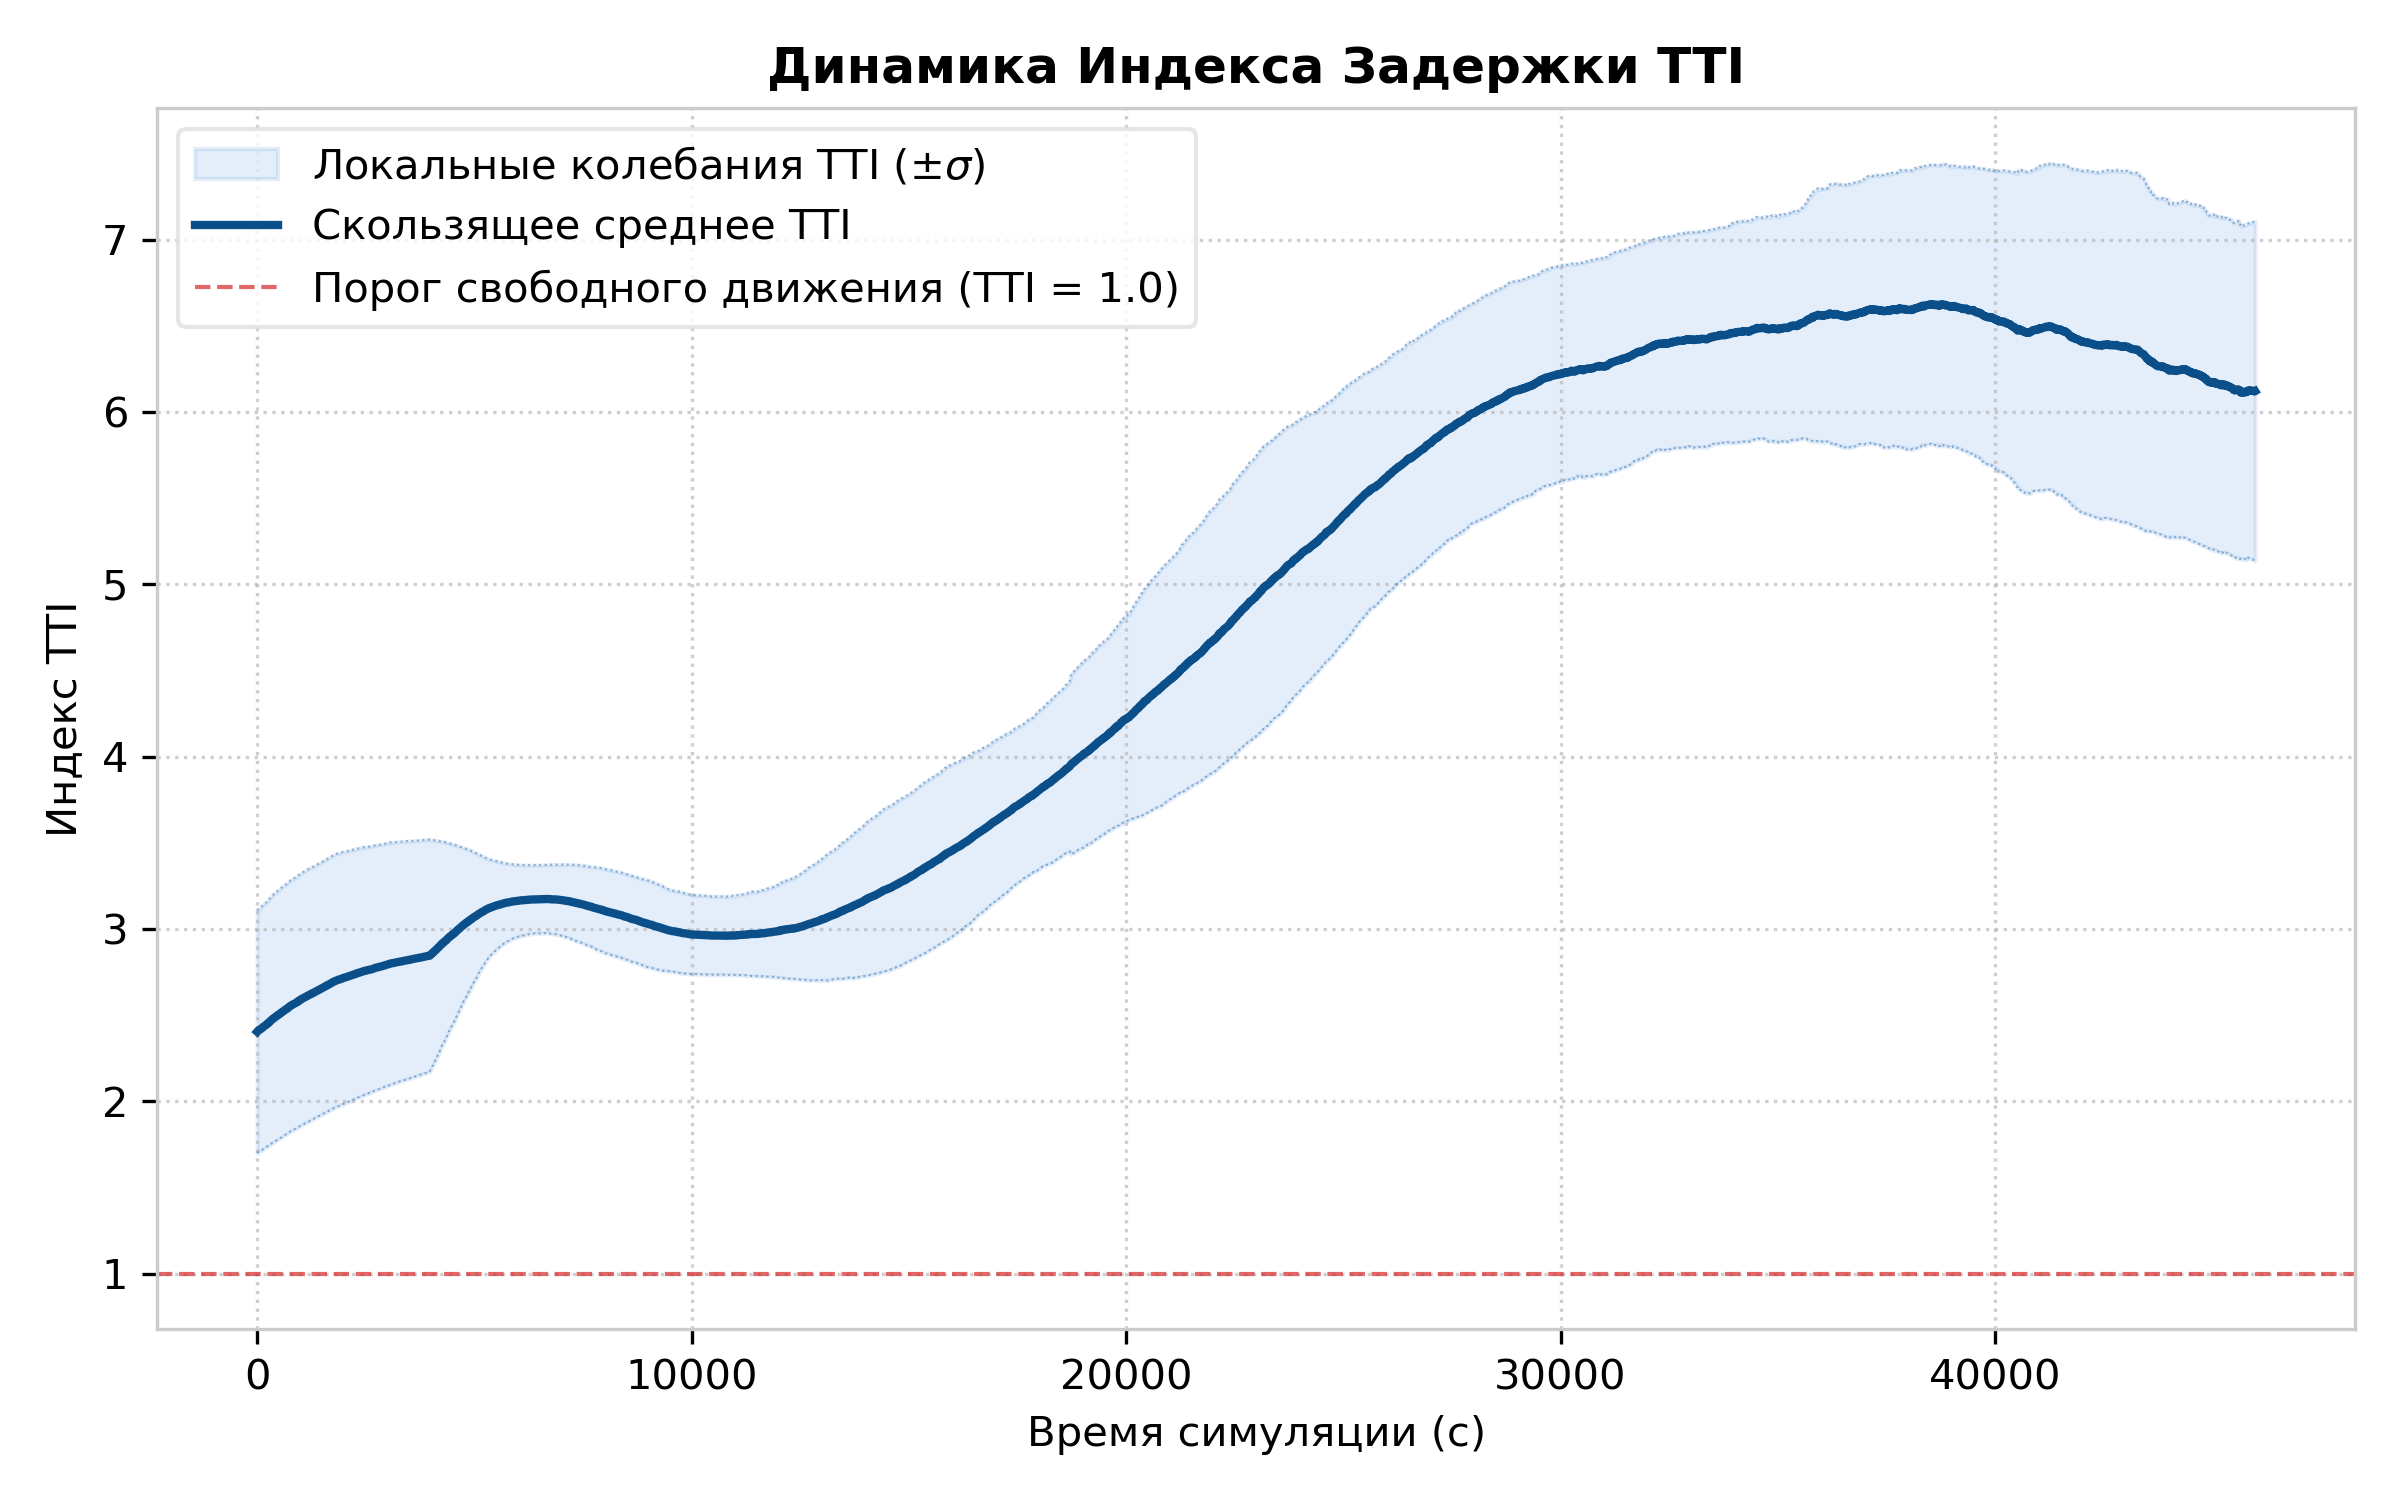
\includegraphics[width=0.85\linewidth,keepaspectratio]{assets/images/fig_tti.png}
    \caption{Динамика Индекса Задержки $TTI$ в ходе симуляции}
    \label{fig:sim_tti}
\end{figure}

\begin{figure}[htbp]
    \centering
    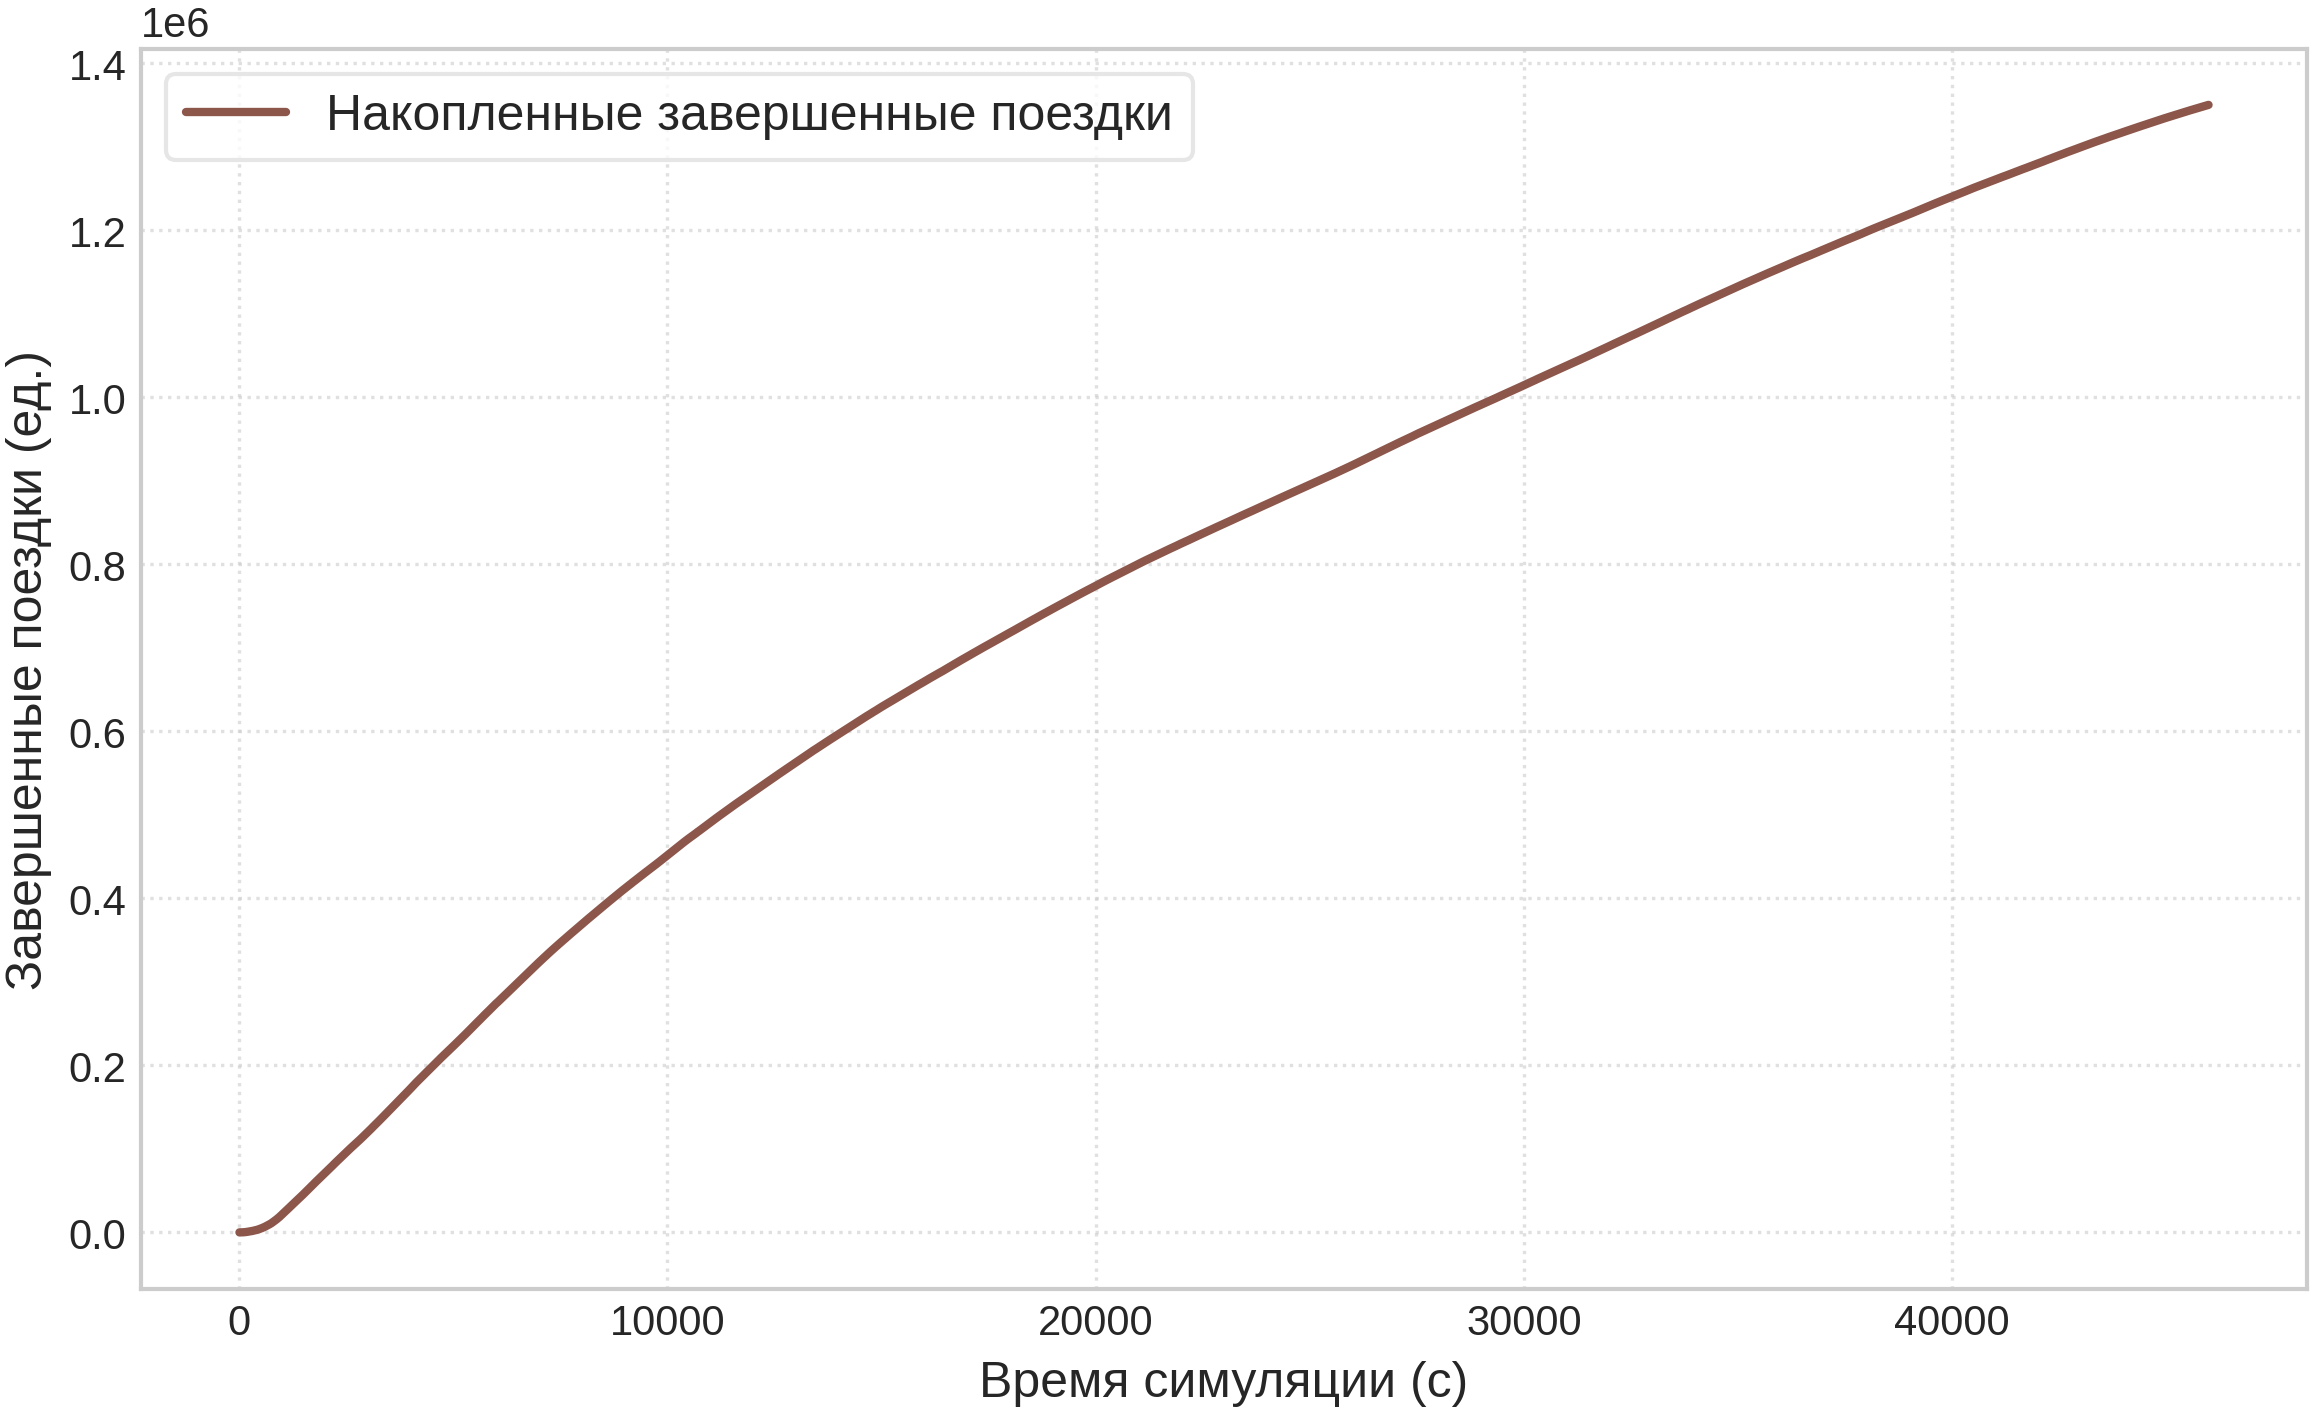
\includegraphics[width=0.85\linewidth,keepaspectratio]{assets/images/fig_completed_trips.png}
    \caption{Интегральная пропускная способность (накопленные завершенные поездки)}
    \label{fig:sim_completed_trips}
\end{figure}

Классификация состояний ребер по плотности и соответствующим им скоростным диапазонам приведена в табл. \ref{tab:traffic_zones}.

\begin{table}[htbp]
    \caption{Классификация состояний ребер дорожного графа по плотности потока}
    \label{tab:traffic_zones}
    \centering
    \begin{tabular}{|l|c|c|p{5.5cm}|}
        \hline
        Цветовая зона & Математическое условие & Скорость $v_{actual}$ & Состояние потока \\ \hline
        Зеленая & $N_{cars} < C_{vis} + 0{,}3(C_{jam} - C_{vis})$ & $> 0{,}97 V_{free}$ & Свободный поток, минимальная задержка \\ \hline
        Желтая & $C_{vis} + 0{,}3(C_{jam} - C_{vis}) \le N_{cars} < C_{jam}$ & $(0{,}83; 0{,}97] V_{free}$ & Плотный поток, возникновение взаимных помех \\ \hline
        Красная & $C_{jam} \le N_{cars} < 2 C_{jam}$ & $[V_{free}/11; 0{,}83] V_{free}$ & Перегрузка, задержка до $10 T_{free}$, скорость падает до $V_{free}/11$ ($5{,}45$~км/ч при лимите $60$~км/ч, $8{,}18$~км/ч при $90$~км/ч) \\ \hline
        Черная & $N_{cars} \ge 2 C_{jam}$ & $0$ & Блокировка ребра ($v_{actual} = 0$), рост обратного затора \\ \hline
    \end{tabular}
\end{table}

Динамика количества свободных ребер (рис. \ref{fig:sim_green_zones}) фиксирует пространственное стягивание потоков. После начального спада количество зеленых ребер кратковременно восстанавливается до $62$~тыс. на $7000$~с, после чего снижается до $27$~тыс. к концу симуляции. В этот же период число перегруженных сегментов в красной и черной зонах суммарно увеличивается с $1210$ до $3578$ (рис. \ref{fig:sim_red_yellow_zones}). Это доказывает, что транспортные средства концентрируются на ограниченном количестве альтернативных маршрутов, полностью исчерпывая их емкость, в то время как остальная часть дорожной сети остается неиспользуемой.

\begin{figure}[htbp]
    \centering
    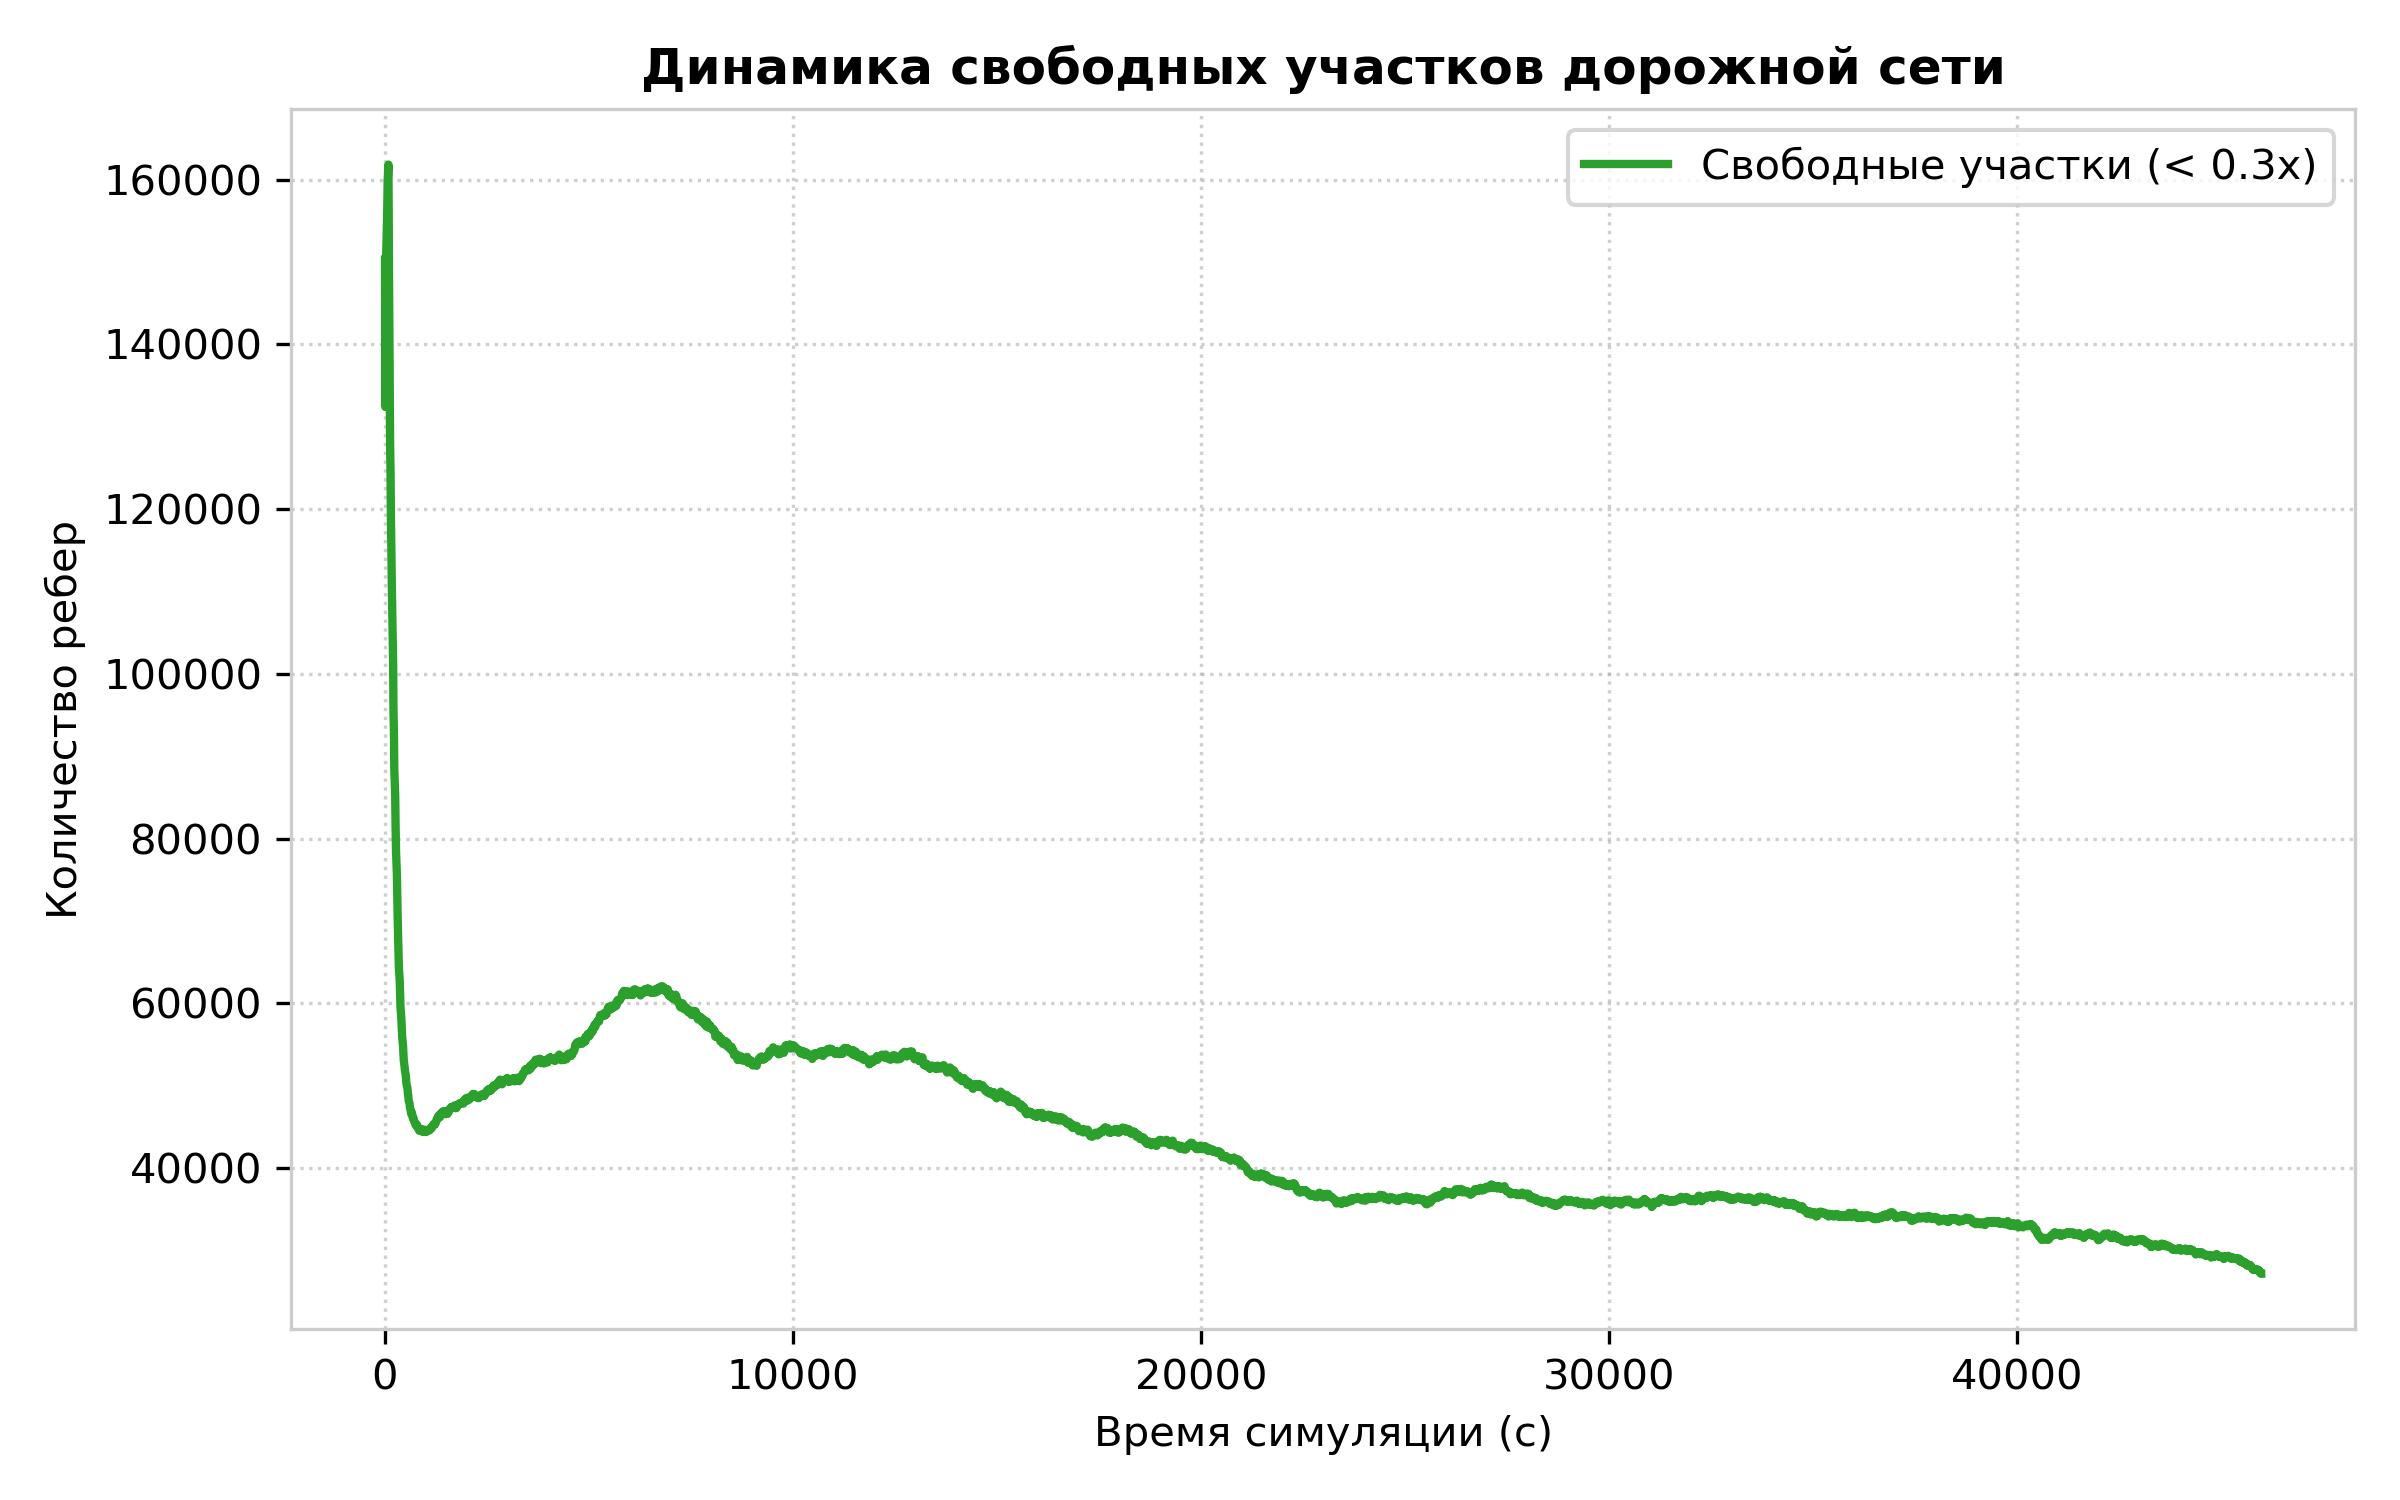
\includegraphics[width=0.85\linewidth,keepaspectratio]{assets/images/fig_green_zones.png}
    \caption{Динамика количества свободных участков дорожной сети}
    \label{fig:sim_green_zones}
\end{figure}

\begin{figure}[htbp]
    \centering
    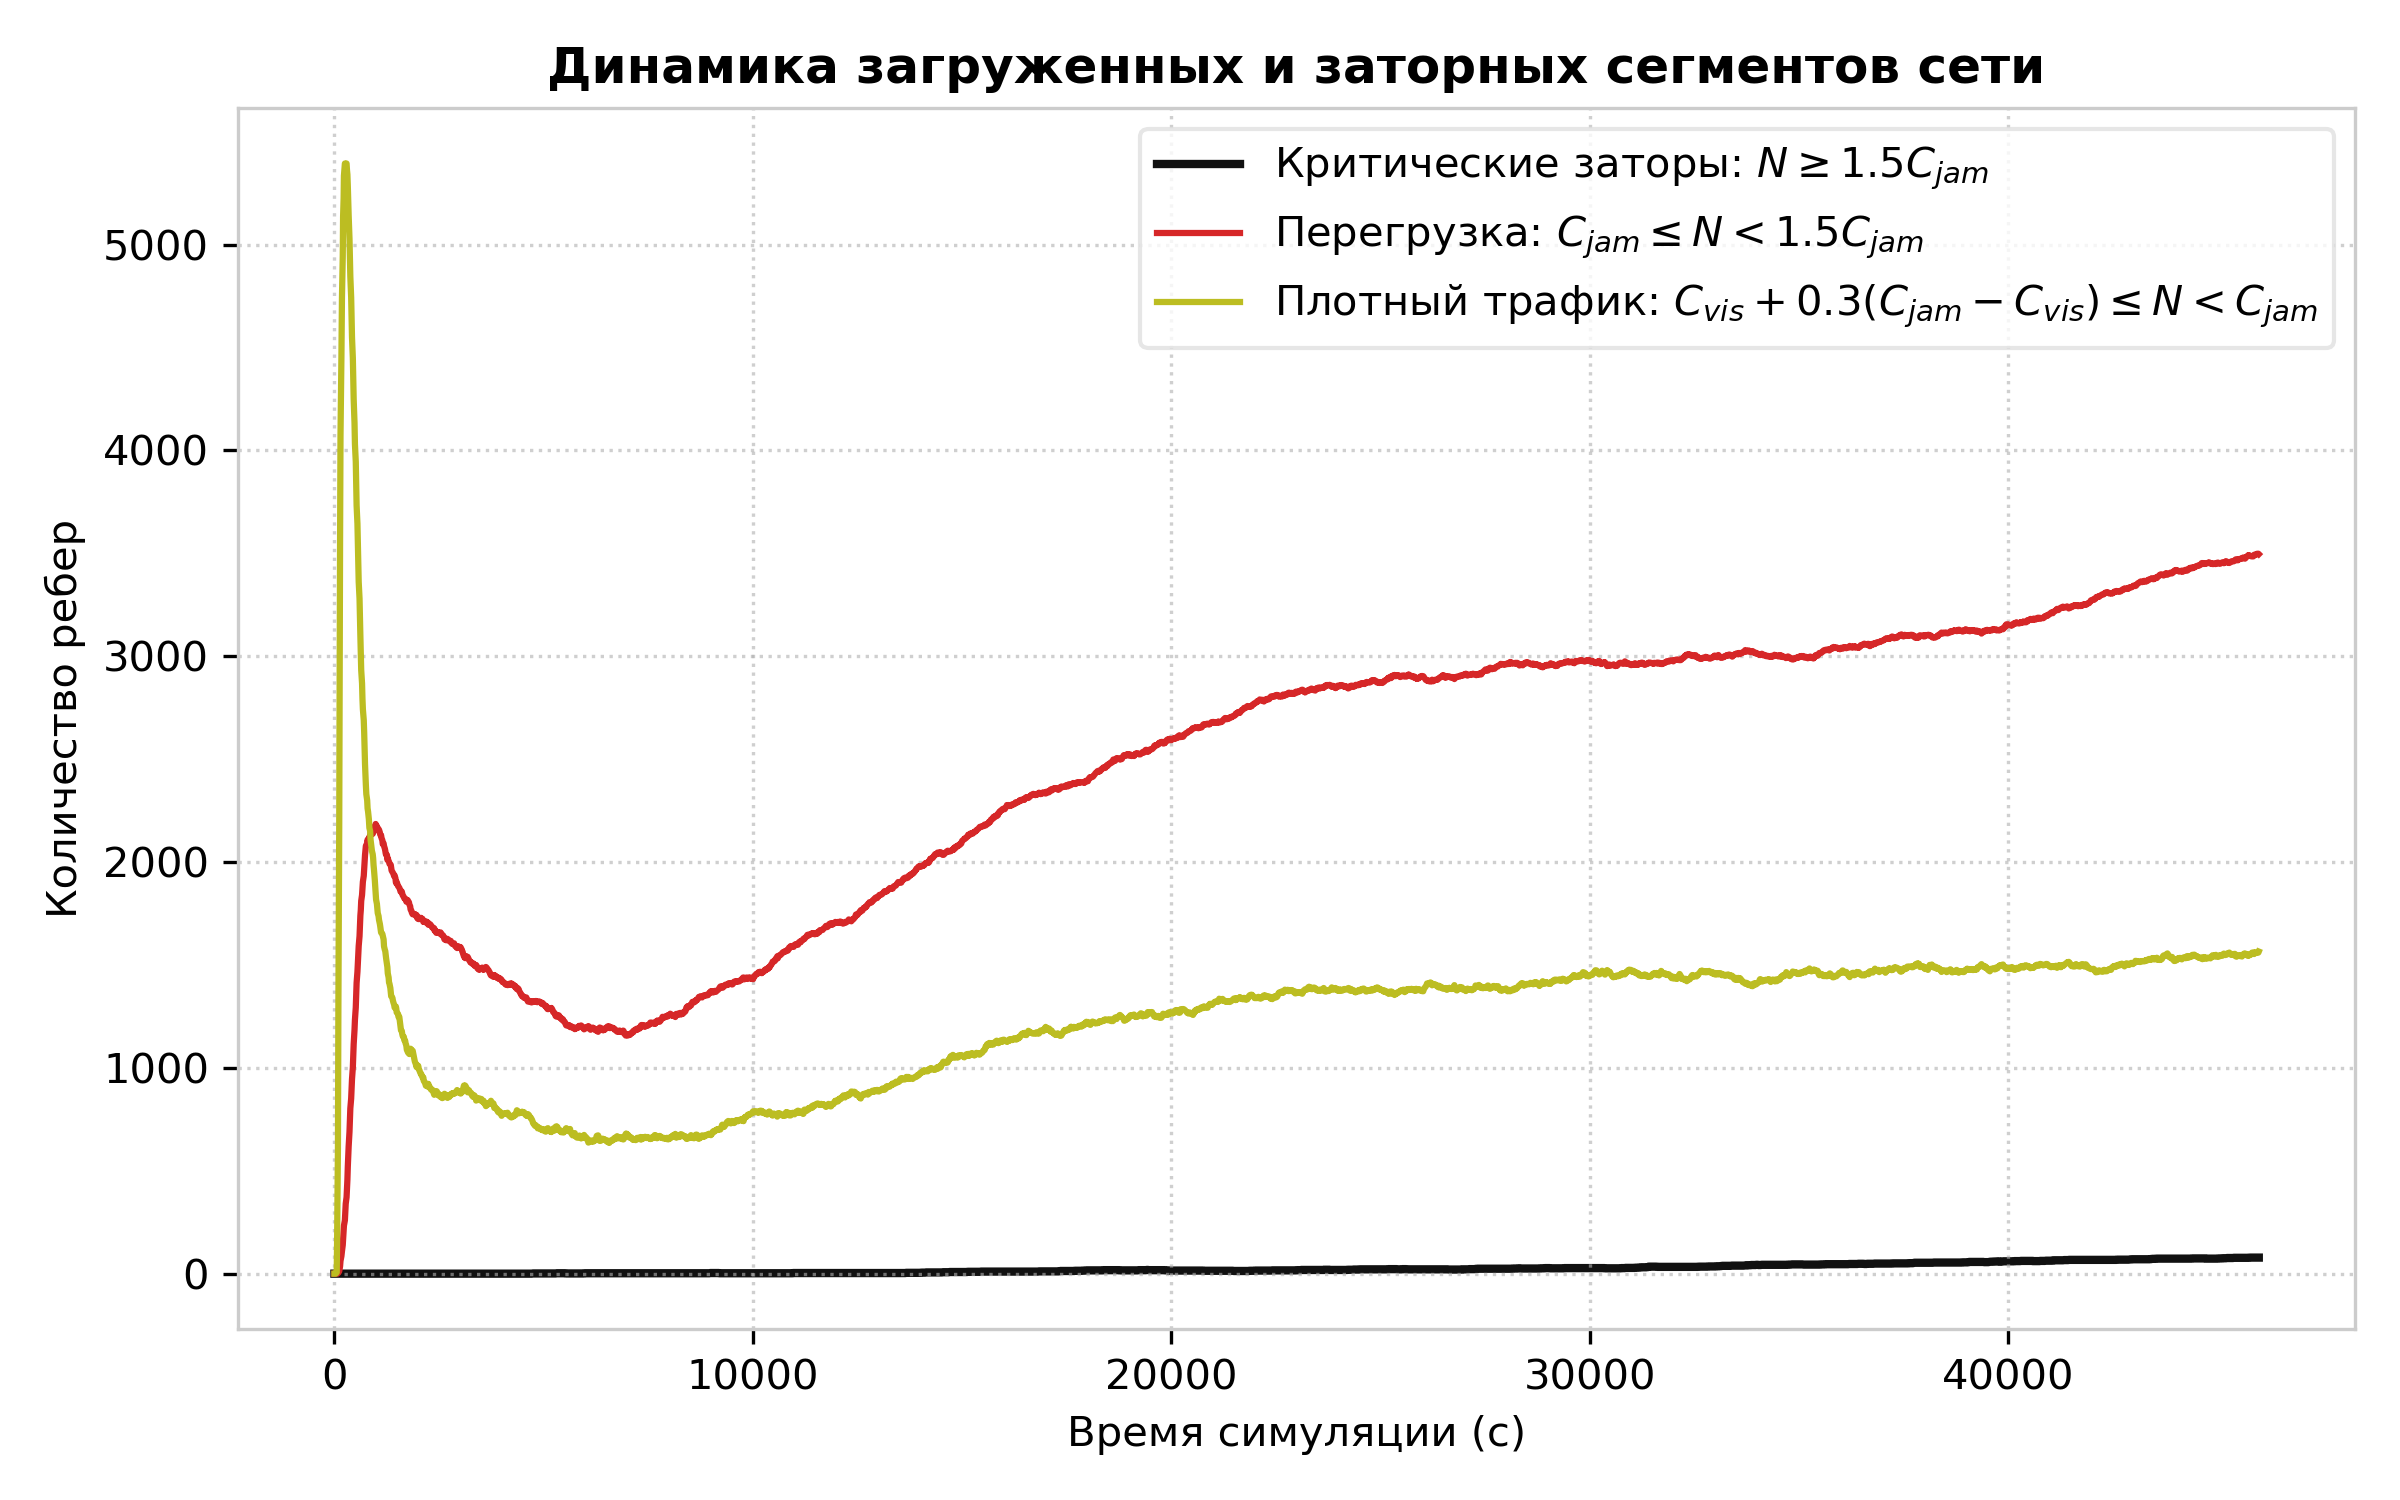
\includegraphics[width=0.85\linewidth,keepaspectratio]{assets/images/fig_red_yellow_zones.png}
    \caption{Динамика загруженных (желтых), перегруженных (красных) и заторных (черных) сегментов сети}
    \label{fig:sim_red_yellow_zones}
\end{figure}

Динамика очередей ожидания маршрутов приведена на рис. \ref{fig:sim_queues}. Очередь выпуска (первичный и повторный старт автомобилей) достигает пика в $81$~тыс. к $7000$~с, снижаясь до $4$~тыс. к концу симуляции. Очередь смены маршрута (запросы на перестроение пути во время движения) достигает максимума в $34$~тыс. к $17~000$~с и стабилизируется на уровне $26$~тыс. машин.

Показатели производительности ядра маршрутизации подтверждают эффективность системы. Средняя скорость обработки запросов (QPS) возрастает с $200$ до $500$ к $8~000$~с, испытывает кратковременное снижение до $400$--$450$ QPS на $11~000$~с (в период перестроения маршрутов), после чего возрастает до пика в $1050$ QPS к концу симуляции. Количество посещенных вершин при поиске пути $A^*$ пикует на уровне $210$ тыс. на $1000$~с, снижаясь до $50$ тыс. вершин к концу симуляции. Среднее время поиска пути снижается с $35$~мс до $9$~мс, хотя максимальное время расчета на сложных маршрутах сохраняет единичные выбросы в диапазоне $100$--$350$~мс. Данные показатели подтверждают, что вычислительное ядро справляется с нагрузкой, а расходимость модели носит транспортно-физический характер.

\begin{figure}[htbp]
    \centering
    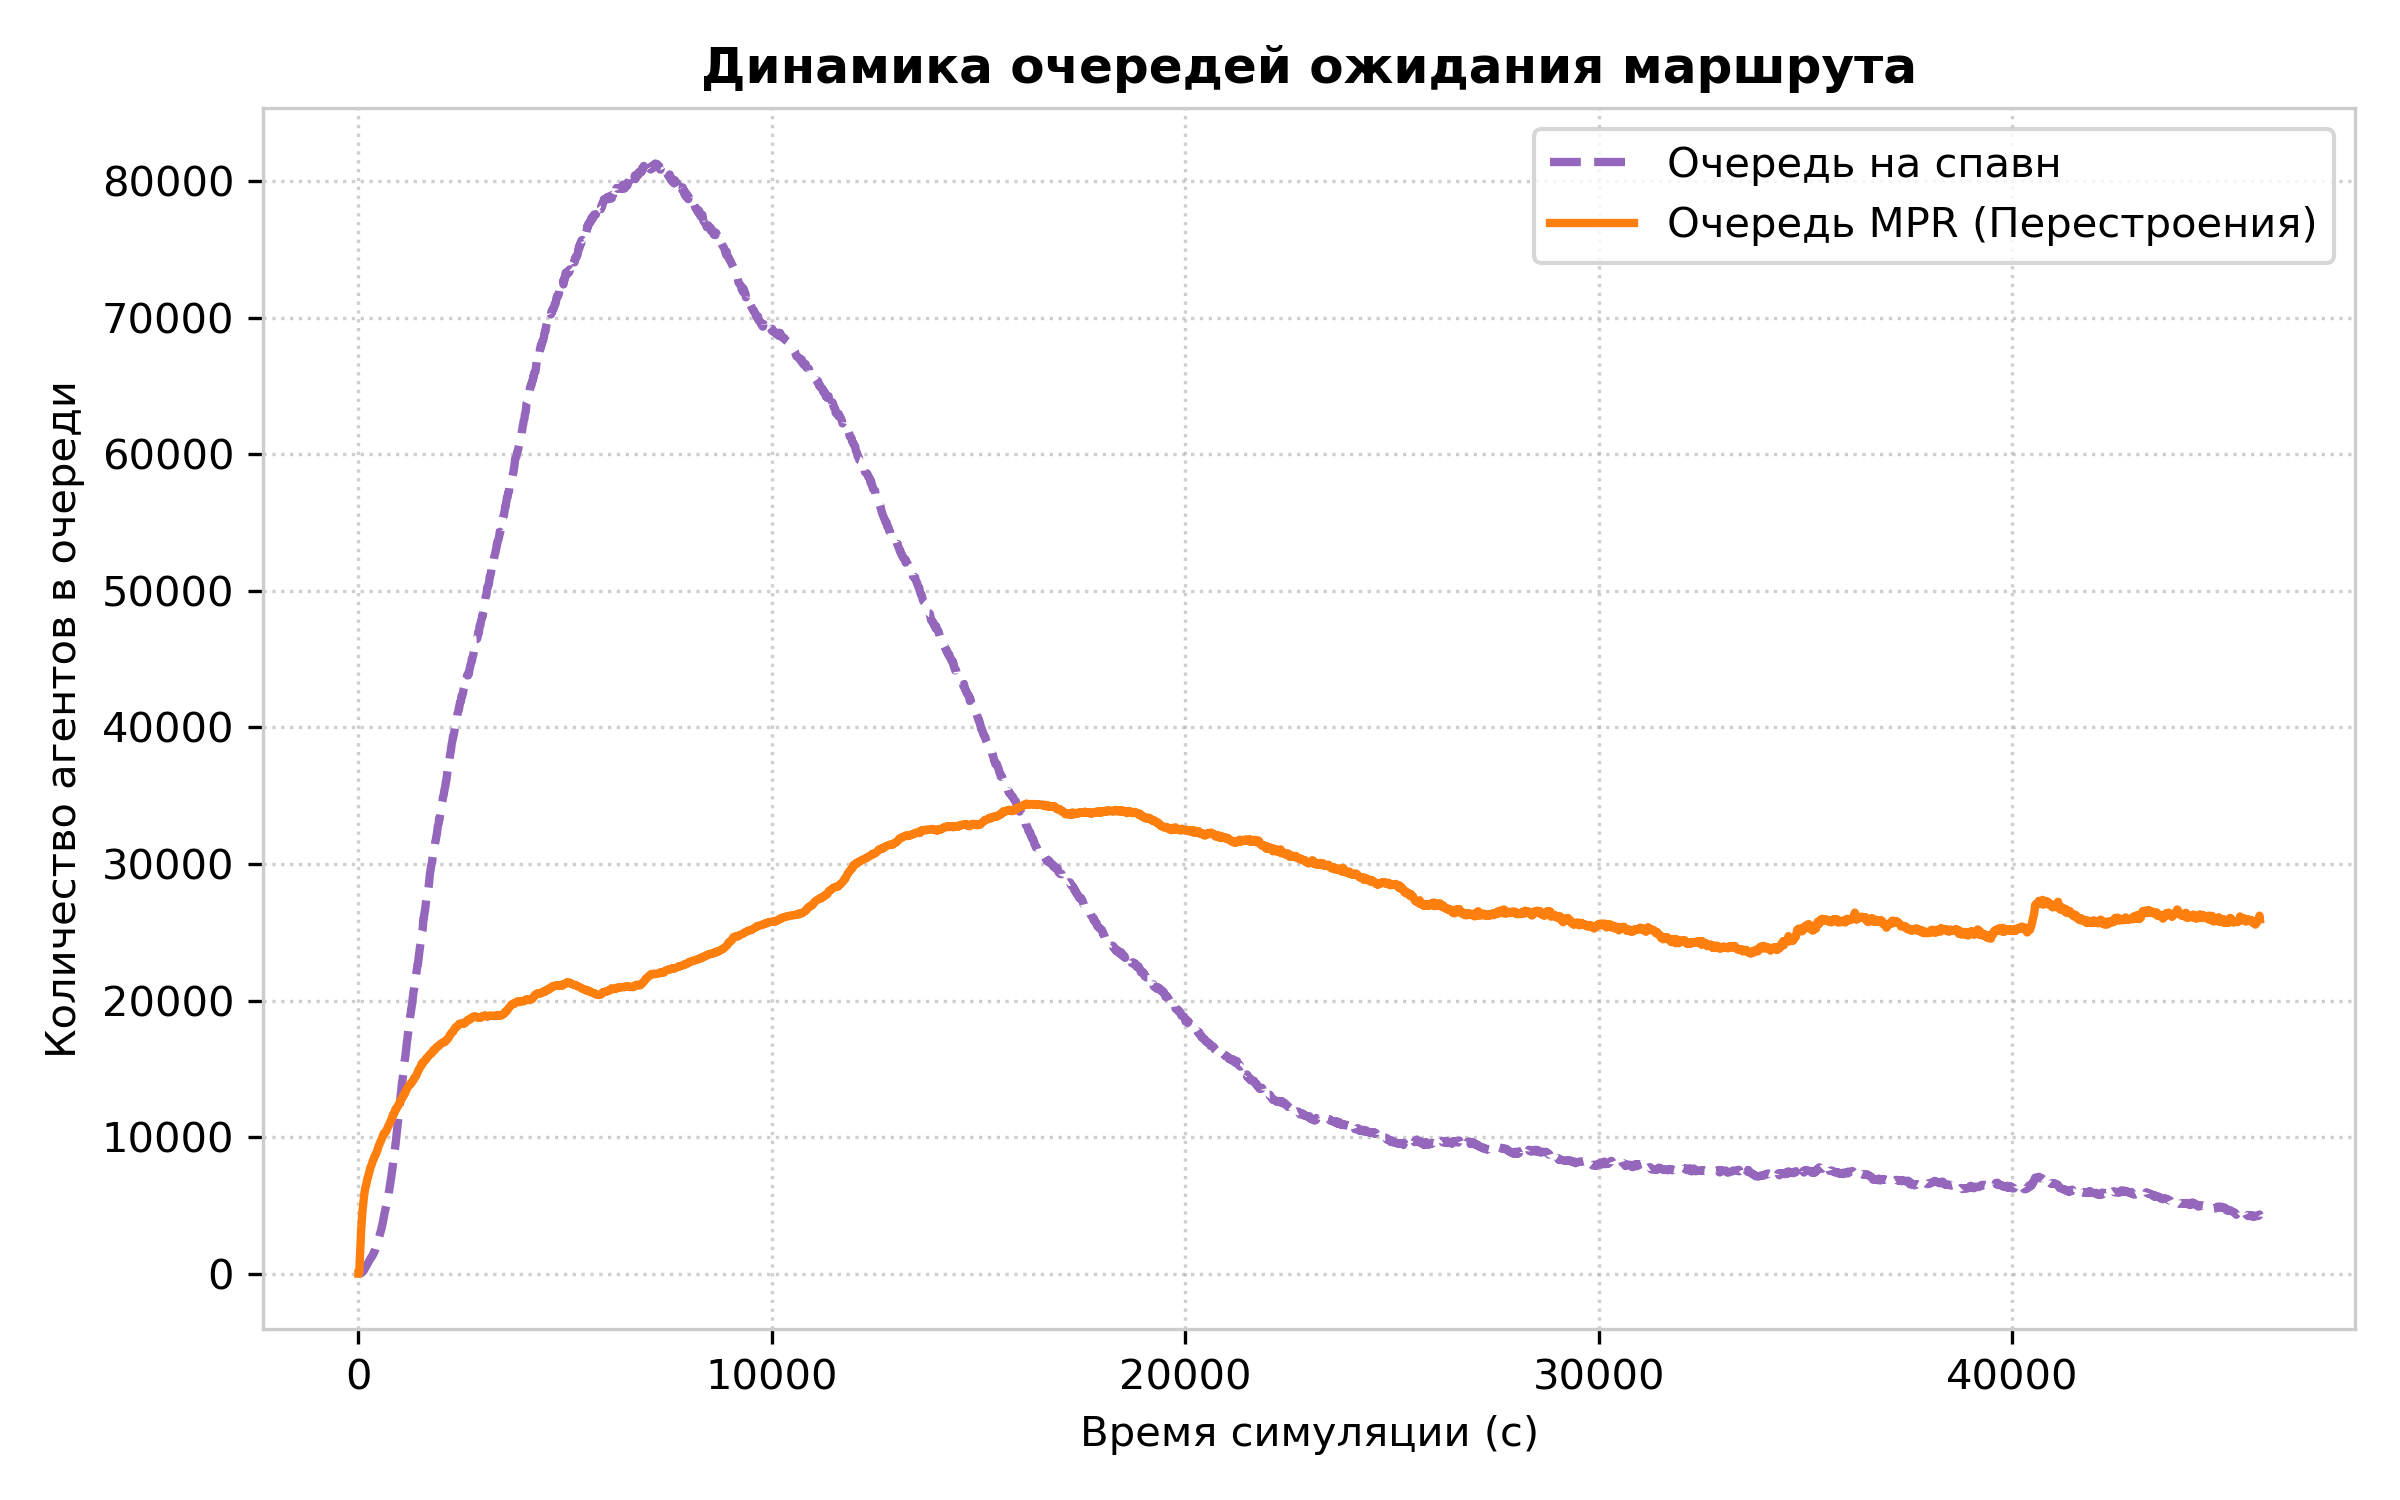
\includegraphics[width=0.85\linewidth,keepaspectratio]{assets/images/fig_queues.png}
    \caption{Динамика очередей ожидания маршрута (первичное появление и перестроения)}
    \label{fig:sim_queues}
\end{figure}

\section{Выводы по третьей главе}
Разработанные низкоуровневые алгоритмы поиска пути и архитектура ядра маршрутизации проверены в ходе экспериментов на субграфе Московской агломерации ($582$~тыс. узлов, $1~460$~тыс. рёбер). Применение метода ориентиров в связке с $8$-арной кучей ускорило поиск пути до $17{,}70$ раз по сравнению с базовым алгоритмом Дейкстры. Привязка потоков к ядрам процессора обеспечила скорость в $5130$ запросов в секунду при работе на $12$ потоках.

Однако интеграционный эксперимент выявил неустойчивость чисто реактивной маршрутизации в условиях запаздывания информации. Полученный отрицательный результат (отсутствие стабилизации TTI) обладает высокой научной ценностью: он строго очерчивает ограничения мезоскопического подхода и доказывает необходимость перехода от реактивного поиска к упреждающему регулированию. В качестве дальнейших направлений исследования предлагается внедрение механизмов мягких штрафов за транзит через потенциально перегружаемые сегменты дорожной сети и алгоритмов распределенной координации потоков на базе графовых нейронных сетей.
